\question{Оптические квантовые генераторы. Лазеры. Условие генерации. 
Пороговый коэффициент усиления.}

Квантовый генератор, или лазер, в отличии от усилителей, является источником
излучения, возбуждаемого непосредственно в нем. Поэтому лазер является
автоколебательной системой с положительной обратной связью, генерация
электромагнитных колебаний в которой осуществляется за счет когерентного
усиления в результате индуцированных переходов.

Необходимая обратная связь в лазере осуществляется за счет помещения рабочей
среды в объемный резонатор. Схема лазера, состоящая из двух необходимых
компонентов~-- активной среды и резонатора, представлена на рис.~\ref{pic12.1}.
Активная среда с инверсной заселенностью 1 обеспечивает усиление за счет
процессов вынужденного излучения. Резонатор условно состоит из плоского
непрозрачного зеркала 2 и параллельного ему полупрозрачного зеркала 3 с
прозрачностью \( \xi \), позволяющего выводить часть излучения наружу.

\begin{figure}[h!]
  \center
  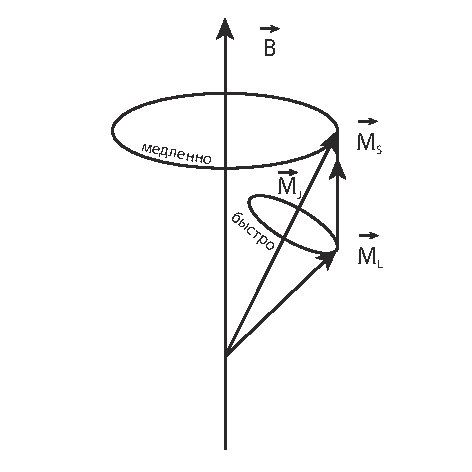
\includegraphics[width=.5\textwidth]{12_01}
  \caption{Принципиальная схема лазера}
  \label{pic12.1}
\end{figure}

Пусть длина активной среды \( L_a \), ее ненасыщенный коэффициент усиления
\( K_0 \) и интенсивность насыщения света \( I_s \); длина резонатора \( L_p \),
общие внутрирезонаторные потери \( \chi = 2L_a\beta_0 \), где \( \beta_0 \)~--
общий коэффициент нерезонаторных потерь.

Порогом генерации является условие превышения усиления электромагнитной волны за
один полный проход резонатора \( e^{2K_0 L_a} \) ее ослабления за счет
внутрирезонаторных потерь \( \chi \) и выхода через полупрозрачное зеркало
\( \xi \). Математически это может быть записано следующим образом:
\[
  e^{2K_\text{п} L_a}(1 - \chi)(1 - \xi) = 1,
\]
где \( K_\text{п} \)~-- коэффициент усиления среды, при котором это происходит.
Его называют пороговым. Как правило \( \chi\xi \ll 1 \), тогда \( K_\text{п} \):
\begin{equation}
  K_\text{п} = \frac{1}{2L_a}\ln\frac{1}{1 - \chi - \xi}.
  \label{eq12.1}
\end{equation}
В отличие от \( K_0 \) пороговый коэффициент усиления является свойством
резонатора, а не активной среды.

Таким образом, если \( K_0 > K_\text{п} \), в лазере начинается стационарная
генерация и излучение электромагнитных колебаний.
